\begin{figure}[tb]
  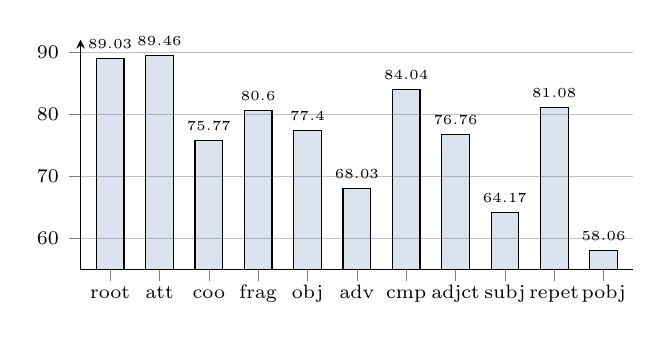
\begin{tikzpicture}
    \begin{axis} [
        width=8.6cm, height=4.5cm,
        ybar,
        axis y line=left,
        axis x line=left,
        x axis line style={-},
        ymajorgrids=true,
        enlarge x limits=0.06,
        tick align=outside,
        ymin=55, ymax=92,
        symbolic x coords={
            root, att, coo, frag, obj, adv, cmp, adjct, subj, repet, pobj
        },
        xtick=data,
        nodes near coords=\pgfmathprintnumber\pgfplotspointmeta,
        xticklabel shift=6,
        x tick label style={anchor=base, font=\scriptsize},
        y tick label style={font=\scriptsize},
    ]
    \addplot [
        draw=black,
        fill opacity=0.2, 
        text opacity=1,
        font=\tiny, 
        fill={rgb,255:red,76; green,114; blue,176}] coordinates {
        (root, 89.03)
        (att, 89.46)
        (coo, 75.77)
        (frag, 80.6)
        (obj, 77.4)
        (adv, 68.03)
        (cmp, 84.04)
        (adjct, 76.76)
        (subj, 64.17)
        (repet, 81.08)
        (pobj, 58.06)
    };
  \end{axis}
\end{tikzpicture}

\caption{
  Accuracy on different dependency labels.
}
\label{fig:model-acc}
\end{figure}
